
% S'exprime dans une dynamique ?
Il y a plusieurs problèmes qui limitent cette possibilité d'une comparaison directe avec les données. Au tout début de notre argumentaire, on a vu avec Hermann que la mobilisation d'un seul critère quantitatif ne pouvait pas suffire à garantir une quelconque explication. Avec suffisament de degrés de liberté, que cela soit par le nombre d'hypothèses mobilisées, ou le nombre de paramètres que l'on met à disposition d'un optimiseur humain ou ordinateur, on trouvera toujours un moyen de se rapprocher des données. \textcite[17]{Amblard2006} parle, par exemple, de surdétermination des paramètres aux données.

%Problème de nature des données, et de leur disponibilités
Un autre problème se pose également avec la mobilisation des données. Du fait de l'\textit{Observational Dilemna}, cette solution d'une comparaison terme à terme explicite entre hypothèses constituantes du modèle et critères n'apparait pas faisable selon \textcite{Batty2001} : \foreignquote{english}{In principle, each element of this process should be explicit and should be capable of being validated with observed data. In practice, this is rarely if ever the case. The data set would be too large, it would be impossible to collect in its entirety, it may be impossible to even observe and measure. Yet the processes are known to be important. Other criteria must thus be used.}

On peut ajouter à cela une autre limite concernant les données, on a en effet vu que toutes les hypothèses d'un modèle n'avaient aucune raison de se placer au même niveau d'abstraction, ou d'appartenir au même formalisme. Il est par exemple déjà difficile d'accéder à des données dans une fenêtre spatio-temporelle donnée, est-il possible d'en avoir sur plusieurs fenêtres, voire plusieurs fenêtres simultanées ?

Le dilemne commence à apparaître clairement, car il ne s'agit pas de tomber dans une \foreignquote{english}{Forrester Strategy}, en abandonnant toute volonté de justifier la chaîne d'hypothèses mobilisées dans les modèles.

% multiplication des critères ?
On peut de nouveau faire appel à l'analyse d'Hermann, dont l'originalité réside aussi dans les remarques très justes et très précoces qu'il a formulées sur la relativité des hypothèses \textbf{mais aussi des critères mobilisés} dans les modèles. Celui-ci est tout à fait conscient qu'il ne s'agit pour l'une comme pour l'autre que d'assertions sur la réalité. Il propose donc d'essayer de faire au mieux. En adoptant une validation multi-critère \Anote{methode_hermann} intégrant les objectifs ayant guidé la construction du modèle, il espère ainsi renforcer le crédit qu'il est possible d'apporter aux simulations, tout en restant sceptique sur la possibilité d'inférer en retour sur les systèmes observés.


\foreignblockquote{english}[\cite{Hermann1967}]{We have arrived at the position, then, that multiple validity criteria are needed because of the error of measurement and because of the recognition that criteria can be only assertions about \enquote{reality}}


Pour \textcite{Amblard2006}, si cette validation externe basée sur une comparaison quantitative avec les données n'est pas impossible, elle n'en reste pas moins difficile à mettre en oeuvre de façon systématique, en partie pour les raisons évoquées ci-dessus. L'appel à des critères d'évaluation plus qualitatifs (\enquote{faits stylisés}) reste le plus évident à mettre en oeuvre. Un point de vue partagé par \textcite{Batty2001}, pour qui \foreignquote{english}{ [...] complex systems models have multiple causes which display a heterogeneity of processes that are impossible to observe in their entirety. The focus is on more qualitative evaluation of a model’s plausibility in ways that relate to prior analysis of the model’s structure.}

Cette démultiplication des critères d'évaluation, même si c'est une opération qui reste indispensable, ne nous sauvera pas d'un autre problème. Il n'y a pas de seuil de suffisance à chercher dans la représentativité des hypothèses, mais également dans leur mise en cohérence/relation, puisque celle-ci tient là encore d'une reconstruction guidée par une but. La recherche d'une cohérence interne au modèle n'apporte pas plus de garantie sur la transférabilité des hypothèses à la réalité. Ce qui ne veut pas dire qu'il ne doit pas y en avoir, seulement celles-ci doivent être faites pour les bonnes raisons, et non pas pour se donner l'illusion d'une meilleure inférence des conclusions du modèle au système observé.

\foreignblockquote{english}[\cite{OSullivan2004}]{There is a many to one relationship between the structure of models and the behaviour they produce, so that many models can account for the same observed outcome. This is the equifinality problem. One common (incorrect) response to the problem is to examine the internal consistency of the model, and to assume that internal consistency guarantees a true representation of reality. Alternatively, we resort to calibration, and adjust model parameters until a best fit to historical data is achieved. Calibration is a complex technical procedure, but ultimately offers no escape. At best, observational data can be replicated more or less closely, but this provides no guarantee as to a model’s accuracy as a representation, nor does it exclude any other model, or another choice of parameters.}

Outre donc la question de la disponibilité des données en sciences humaines et sociales, l'\textit{Observational Dilemna} sous-tend également l'impossibilité d'établir l'unicité des hypothèses avancées pour décrire un phénomène, mais aussi par extension celle des critères d'évaluation, qui restent eux aussi des construits formulés sur la base d'une observation du système observé. Capturer toute la substance d'un phénomène émergent dans un ou plusieurs critères d'évaluation reste difficile, voire impossible.

Cette variabilité exprimée dans la construction et la paramétrisation des structures causales et des critères associés renvoie à ce phénomène bien connu des modélisateurs en sciences humaines et sociales, à savoir l'équifinalité (voir la figure \ref{fig:S_equifinalite}).

\begin{figure}[htbp]
\begin{sidecaption}[Schéma de représentation de l'équifinalité]{Schéma de représentation de l'équifinalité, inspiré de \autocite{Richardson2002} : \foreignquote{english}{Illustration showing that not only can a particular system state (outcome) can be reached via different trajectories from the same starting conditions, but also that different starting conditions may also lead to the same system state. Of course, the reverse case is also a possibility in that different starting conditions may lead to different outcomes and multiple runs from the same starting conditions may also result in different outcomes.}}[fig:S_equifinalite]
  \centering
 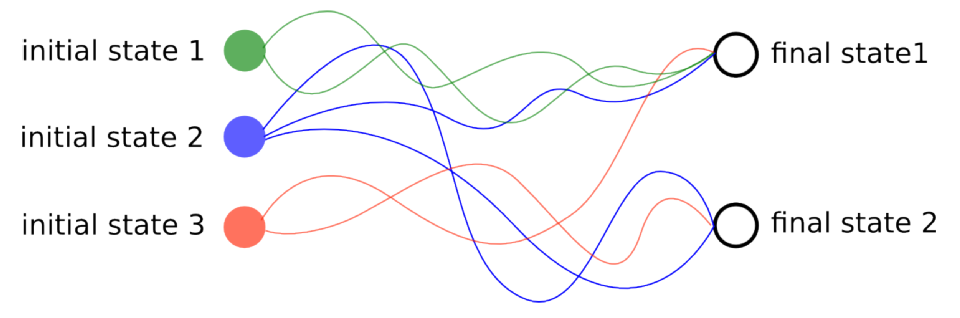
\includegraphics[width=.9\linewidth]{equifinalite.png}
  \end{sidecaption}
\end{figure}

L'équifinalité est un concept provenant à l'origine d'un phénomène observé en embryologie \Anote{embryon}, généralisé ensuite par Bertalanffy comme \textbf{une propriété fondamentale des systèmes ouverts} (voir la section \ref{subsec:gst} en annexe pour une remise en contexte du terme). Celui-ci reste un terme couramment employé dans la littérature, et que l'on retrouve associé à une limitation dans la \enquote{Vérification} \Anote{verification_philo} en philosophie :

\foreignblockquote{english}[\cites{OSullivan2004,Oreskes1994}]{\textcite{Oreskes1994} crisply describe the problem: it is impossible to verify the representational truth of any model of an open system. There is a many to one relationship between the structure of models and the behaviour they produce, so that many models can account for the same observed outcome. This is the equifinality problem.}
